% ============================================================
%  DOCUMENTO LaTeX
%  Título: Modelo de transformación cuántica variacional de
%          características de cáncer de mama para un sistema
%          híbrido de prediagnóstico
%  Instituto: Instituto Politécnico Nacional — ESCOM
%  TT No. 2026 – B039
% ============================================================

% ------------------------------------------------------------
% PREÁMBULO — paquetes y configuración general
% ------------------------------------------------------------
\documentclass[12pt, letterpaper]{article}

% Codificación y lenguaje
\usepackage[utf8]{inputenc}
\usepackage[T1]{fontenc}
\usepackage[spanish]{babel}

% Tipografía — compatible con pdflatex
\usepackage{lmodern}           % Fuente moderna con soporte completo de caracteres

% Márgenes y geometría de página
\usepackage[
  top=2.54cm,
  bottom=2.54cm,
  left=2.54cm,
  right=2.54cm
]{geometry}

% Interlineado
\usepackage{setspace}
\setstretch{2}                 % Doble espacio (equivalente al documento original)

% Imágenes y gráficos
\usepackage{graphicx}
\usepackage{float}

% Hipervínculos y tabla de contenidos
\usepackage{hyperref}
\hypersetup{
  colorlinks = true,
  linkcolor  = black,
  urlcolor   = blue,
  citecolor  = black
}

% Numeración de figuras por subsección
\usepackage{amsmath}
\numberwithin{figure}{subsection}

% Tablas
\usepackage{booktabs}
\usepackage{array}
\usepackage{tabularx}

% Espaciado entre párrafos
\usepackage{parskip}
\setlength{\parindent}{0pt}

% Encabezados de sección sin numeración automática en índice
\usepackage{titlesec}

% Bibliografía y citas con hipervínculos
\usepackage{url}
\usepackage[numbers, square]{natbib}   % Citas numéricas estilo [1], [2], etc.
% NOTA: hyperref + natbib hacen que el número sea un hipervínculo automáticamente.

% Líneas divisoras — comandos personalizados
% Uso: \divider          → línea fina al ancho del texto
% Uso: \dividerthick     → línea más gruesa
\newcommand{\divider}{%
  \vspace{0.8em}%
  \noindent\rule{\linewidth}{0.4pt}%
  \vspace{0.8em}%
}
\newcommand{\dividerthick}{%
  \vspace{0.8em}%
  \noindent\rule{\linewidth}{1.2pt}%
  \vspace{0.8em}%
}

% ------------------------------------------------------------
% INICIO DEL DOCUMENTO
% ------------------------------------------------------------
\begin{document}

% ============================================================
% PORTADA
% ============================================================

% --- Logos institucionales ---
\begin{figure}[H]
  \centering
  % Logo izquierdo (ESCOM / IPN)
  \begin{minipage}{0.30\textwidth}
    \centering
    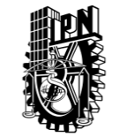
\includegraphics[width=\linewidth]{Logos/IPN_logo.png}  % Reemplazar con la imagen real
  \end{minipage}
  \hfill
  % Logo derecho (ESCOM)
  \begin{minipage}{0.30\textwidth}
    \centering
    
\includegraphics[width=\linewidth]{Logos/ESCOM_logo.png}  % Reemplazar con la imagen real
  \end{minipage}
\end{figure}

\vspace{1em}

% --- Institución y programa ---
\begin{center}
  {\large \textbf{INSTITUTO POLITÉCNICO NACIONAL}}\\[0.5em]
  {\large \textbf{Escuela Superior de Cómputo}}\\[0.5em]
  {\large \textit{Licenciatura en Ciencia de Datos}}\\[1em]
  TT No. 2026 -- B039\\[1em]
  ``Modelo de transformación cuántica variacional de características de cáncer
  de mama para un sistema híbrido de prediagnóstico''\\[3em]
\end{center}

\vspace{1.5em}

% --- Tabla de presentadores y directores ---
\begin{center}
  \begin{tabular}{p{0.42\textwidth} p{0.10\textwidth} p{0.42\textwidth}}
    \textbf{Presenta}: & & \textbf{Directores}: \\[0.4em]
    Miguel Alexander Sánchez García
    & &
    Dra. Ana María Winfield Reyes \\
    & & Dr. Jesús Yaljá Montiel Pérez \\
  \end{tabular}
\end{center}

% ============================================================
% TABLA DE CONTENIDOS (ÍNDICE)
% ============================================================
\newpage
\tableofcontents

% ============================================================
% SECCIÓN: RESUMEN
% ============================================================
\newpage
\section*{Resumen}
\addcontentsline{toc}{section}{Resumen}

% [Contenido del resumen — pendiente de redacción]

% ============================================================
% SECCIÓN: ABSTRACT
% ============================================================
\newpage
\section*{Abstract}
\addcontentsline{toc}{section}{Abstract}

% [Contenido del abstract — pendiente de redacción]

% ============================================================
% SECCIÓN 1 — PANORAMA GENERAL
% ============================================================
\newpage
\section{Panorama General}

% ------------------------------------------------------------
% 1.1 Introducción
% ------------------------------------------------------------
\subsection{Introducción}
% ----------------------------------------------------------
% 1.1.1 Contexto clínico del cáncer de mama
% ----------------------------------------------------------
\subsubsection{Contexto clínico del cáncer de mama}

El cáncer de mama es una enferdad caracterizada pro la proliferación descontrolada de células en el tejido mamario, que forma tumores malignos con capacidad de expandirse sistemáticamente si no recibe tratamiento oportuno. A nivel mundial, constituye el cáncer más frecuente diagnosticado en mujeres y la principal causa de muerte por cáncer femenino, superando incluso el cáncer de pulmón en incidencia global.

Según los datos de GLOBOCAN 2022 de la Agencia Internacional para la Investigación sobre el Cáncer (IARC), en 2022 se registraron aproximadamente 2.3 millones casos nuevos de cáncer de mama y una mortalidad de alrededor de 670,000 mujeres a nivel mundial \cite{GLOBOCAN2022}. El cáncer de mama representa actualmente uno de cada cuatro cánceres en mujeres a nivel global, y desde 2008 la incidencia mundial ha aumentado más de 20\%, mientras que la mortalidad se ha incrementado en un 14\% \cite{BCRF2025}. Las proyecciones son igualmente preocupantes: si las tasas nacionales actuales se mantienen estables, para 2050 el número de casos nuevos y defunciones por cáncer de mama a nivel mundial aumentará más de 50\% y 70\% respectivamente, impulsando principalmente por el crecimiento y envejecimiento de la población \cite{StopBreastCancer2025}

Las disparidades regionales son significativas y tienen implicaciones directas para el desarrollo de herramientas de diagnóstivo asistido. En paises de bajos ingresos, la tasa de mortalidad por cáncer de mama puede ser el doble que en países más desarrollados, a pesar de tener una incidencia considerablemente menor, lo que refleja la falta o inadecuada infraestructura de servicios de detección temprana y tratamiento oportuno \cite{GlobalCancerStatistics2024}. Esta brecha evidencia que el problema no es unicamente epidemiológico, sino tambien tecnológico y de acceso a herramientas diagnósticas.

\textbf{Panorama en México}{}

En el contexto nacional, la situación es igualmente urgente. Según datos del Instituto Nacional de Estadística y Geografía (INEGI), en 2024 el cáncer de mama fue la principal causa de muerte por tumores malignos en México, con aproximadamente 8,500 defunciones registradas, de los cuales el 99.2\% correspondieron a mujeres, con una tasa de mortalidad de 18.7 por cada 100,000 mujeres de 20 años o más \cite{CancerMexico2025}. Este indicador refleja un deterioro; durante la última década, la tasa de defunciones por cáncer de mama se incrementó de 15.7 en 2015 a 18.7 en 2024 por cada 100,000 mujeres de 20 años o más. \cite{INEGI2025}

% Figura 1.1.1 — Incidencia y mortalidad por cáncer de mama en México (INEGI 2025)
\begin{figure}[H]
  \centering
  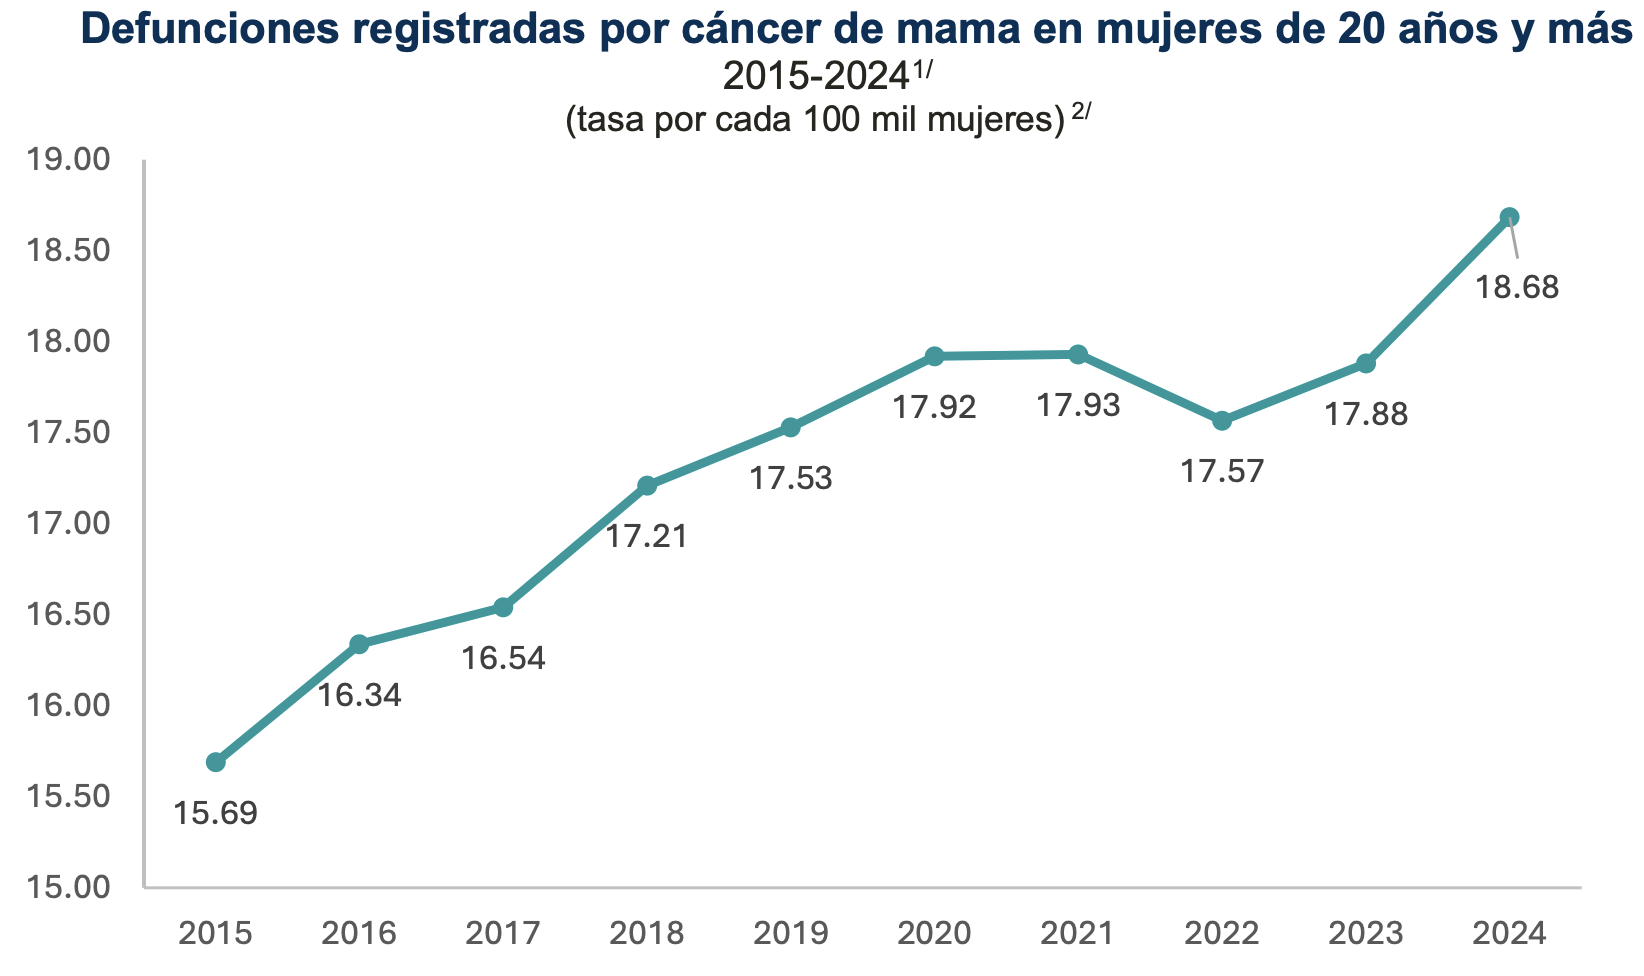
\includegraphics[width=0.65\textwidth]{Figures/Figura_1_1_1.png}
  \caption{Incidencia y mortalidad por cáncer de mama en México (INEGI 2025) \cite{INEGI2025}}\label{fig:MexicoBreastCancerStats}
\end{figure}

A nivel estatal, la distribución es heterogénea, siendo Chihuahua y Baja California Sur los estados con mayor tasa de mortalidad, mientras que Guerrero y Tlaxcala registran las tasas más bajas. Por grupo de edad, el segmento más afectado es el de mujeres entre 50 y 59 años.

% Figura 1.1.1 — Incidencia y mortalidad por cáncer de mama en México (INEGI 2025)
\begin{figure}[H]
  \centering
  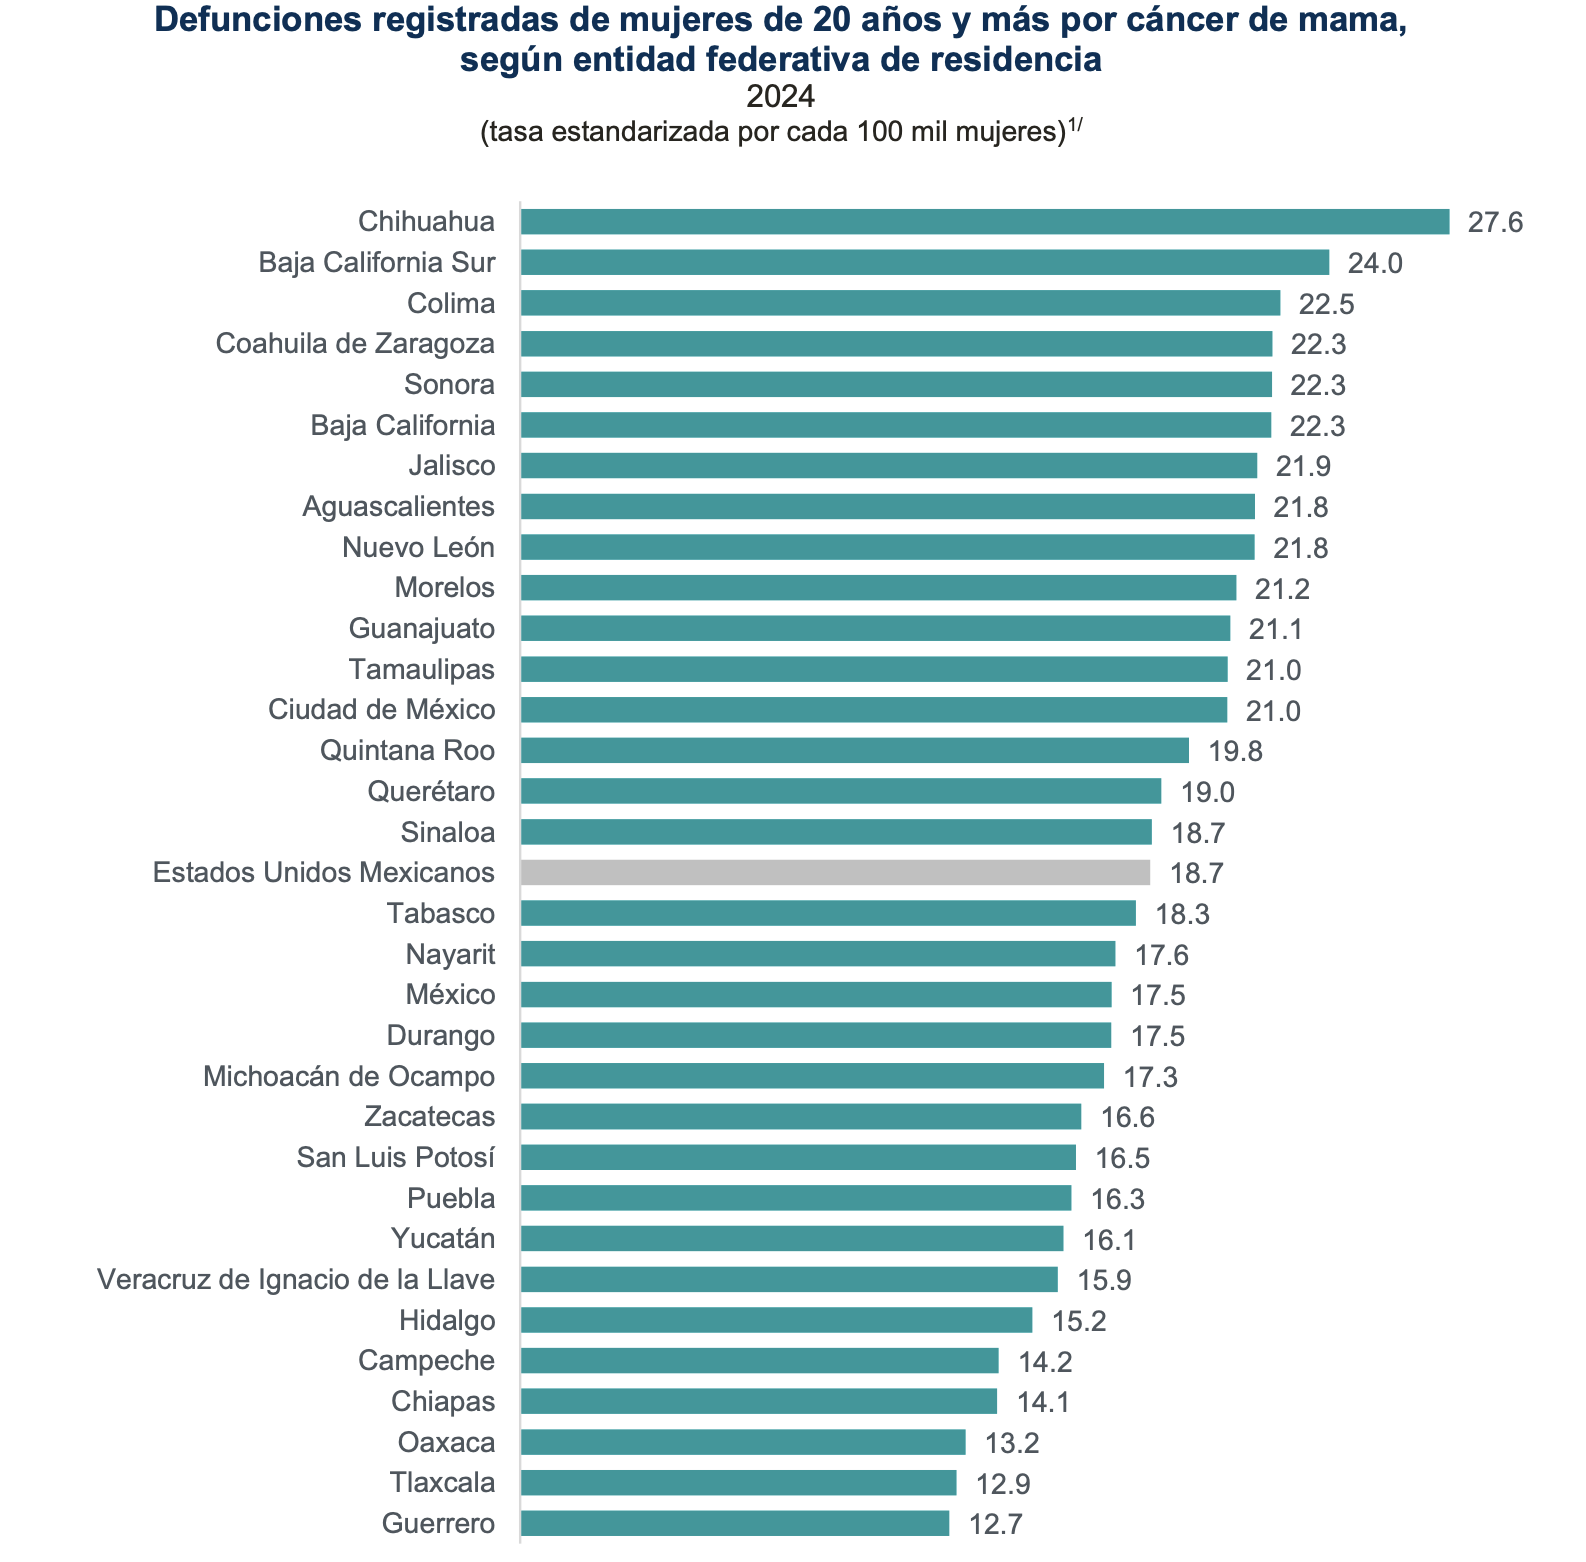
\includegraphics[width=0.6\textwidth]{Figures/Figura_1_1_2.png}
  \caption{Incidencia y mortalidad por cáncer de mama en México por Estado (INEGI 2025) \cite{INEGI2025}}\label{fig:MexicoBreastCancerStats}
\end{figure}

\textbf{La detección temprana como factor determinante}{}

El elemento clínico más relevante para justificar el desarrollo de sistemas de prediagnóstivo automatizado es el impacto radical de la detección temprana sobre la supervivencia. Según la American Cancer Society, cuando el cáncer de mama se detecta en etapa temprana y se encuentra en una fase localizada, la tasa de supervicencia relativa a cinco años es del 99\% \cite{NBCF2026_EarlyDetection}. Esta cifra contrasta drásticamente con los casos en etapa avanzada con metastátis, donde la supervivencia a cinco años cae a 30\%. Las mujeres que reciben tamizaje regular de cáncer de mama presentan una tasa de mortalidad de un 26\% menor que las que no se somente a cribado.

La mamografía es el instrumento central de detección temprana. Es el único método de tamizaje demostrado para reducir las muertes por cáncer de mama según el American College of Radiology, y las tasas de mortalidad por esta enfermedad disminuyeron un 42\% entre 1989 y 2021, en parte gracias a la detección temprana mediante cribado mamográfico. \cite{Windsong2026_EarlyDetection}. Sin embargo, la interpretación manual de mamografías presenta limitaciones inherentes: la variabilidad inter-observador entre radiólogos, la dificultad de detección en tejidos de alta densidad mamaria, y la carga de trabajo creciente en los sistemas de salud constituyen factores que motivan el desarrollo de sistemas de diagnóstico asistido por computadora (CADx).

En México, la disponibilidad de infraestructura diagnóstica sigue siendo un desafío. En 2021 se registraron 1,281 mastógrafos en el país, de los cuales 41.1\% se encontraba en instituciones de salud y seguridad social, 36.1\% en establecimientos particulares y 22.8\% en servicios para población sin derechohabiencia \cite{INEGI2023}. Esta distribución limitada, combinada con el incremento sostenido en la mortalidad, subraya la necesidad de desarrollar herramientas tecnológicas que amplíen la capacidad diagnóstica del sistema de salud, haciendo más eficiente y accesible la interpretación de estudios mamográficos.

Es en este contexto donde el presente trabajo propone explorar el uso de transformaciones cuánticas variacionales sobre características extraídas de mamografías del dataset CBIS-DDSM, con el fin de evaluar si estas representaciones mejoran la separación de clases benigno/maligno cuando se integran como entrada de una red neuronal clásica, contribuyendo al desarrollo de herramientas de prediagnóstico asistido más robustas.


% ----------------------------------------------------------
% 1.1.2 Limitaciones de los métodos clásicos de diagnóstico asistido
% ----------------------------------------------------------
\subsubsection{Limitaciones de los métodos clásicos de diagnóstico asistido}

El diagnóstico asistido por computadora (CADx) en mamografía ha experimentado un notable desarrollo durante las últimas dos décadas, impulsado principalmente por el avance de las redes neuronales convolucionales (CNN) y las técnicas de deep learning. No obstante, a pesar de los resultados prometedores reportados en condiciones controladas, estos métodos presentan limitaciones estructurales que restringen su aplicabilidad clínica generalizada.

\textbf{Variabilidad e inconsistencia diagnóstica}{}

La interpretación manual de mamografías está sujeta a una variabilidad inherente entre radiólogos. La variabilidad entre lectores y la dificultad intrínseca de interpretar características radiográficas sutiles limitan con frecuencia la precisión del diagnóstico mamográfico \cite{GlobalCancerStatistics2024_2}, lo que motivó el desarrollo de sistemas CADx automatizados. Sin emabargo, los modelos de deep learning han heredado parte de esta inconsistencia de una forma distinta: en lugar de variar entre observadores humanos, varían entre conjuntos de datos.

El estudio de Wang et al. (2020), publicado en el Journal of the American College of Radiology, es uno de los trabajos más citados al respecto. Los tres modelos publicados con alto rendimiento reportaron puntuaciones AUC-ROC de validación entre 0.88 y 0.95 en el conjunto de datos de entrenamiento; sin embargo, al evaluarse sobre tres conjuntos de datos externos, el rendimiento de los seis modelos disminuyó significativamente, obteniéndose valores de AUC-ROC de apenas entre 0.44 y 0.65. Este hallazgo es especialmente relevante para la presente investigación, ya que demuestra que el alto rendimiento de un modelo de deep learning en un dataset específico no garantiza su transferibilidad a datos con distribuciones distintas, una condición inevitable en entornos clínicos reales donde los equipos de adquisición, las poblaciones de pacientes y los protocolos de imagen varían considerablemente.

\textbf{Limitaciones de interpretabilidad}{}

Es importante abordar los desafíos asociados a la implementación de deep learning en entornos clínicos; la investigación futura debe enfocarse en mejorar la interpretabilidad de los modelos y garantizar su generalización para integrar exitosamente el diagnóstico asistido por deep learning en programas rutinarios de tamizaje de cáncer de mama. \cite{Kim2025GlobalBreastCancer}. La naturaleza de caja negra de las CNN profundas genera desconfianza clínica, ya que los radiólogos no pueden verificar el razonamiento que conlleva a una predicción, lo cual es un requisito indispensable para cualquier herramienta de apoyo a la decisión médica.

\textbf{Alta dimensionalidad y representación de características}{}

Desde una perspectiva de ciencia de datos, los métodos clásicos enfrentan el desafío de la alta dimensionalidad de las imágenes mamográficas. El sobreajuste ocurre cuando los modelos aprenden demasiado bien los detalles de los datos de entrenamiento pero no generalizan adecuadamente para realizar buenas predicciones sobre datos no vistos, lo que sucede típicamente cuando el tamaño del conjunto de entrenamiento es demasiado pequeño en comparación con el número de parámetros del modelo que deben aprenderse. Las técnicas de aumento de datos y regularización mitigan parcialmente este problema, pero no lo resuelven de forma fundamental, especialmente en datasets de tamaño moderado como el CBIS-DDSM.

En conjunto, estas limitaciones evidencian la necesidad de explorar nuevos paradigmas de representación de datos que superen las restricciones del aprendizaje clásico, particularmente en lo que respecta a la separabilidad de características en espacios de alta dimensión.

% -----------------------------------------------------------
% 1.1.3 Computación cuántica como alternativa
% -----------------------------------------------------------
\subsubsection{Computación cuántica como alternativa}

Ante las limitaciones descritas, la computación cuántica emerge como un paradigma complementario que ofrece mecanismos cualitativamente distintos para la representación y transformación de datos clínicos. Su propuesta central no es sustituir a los métodos clásicos, sino enriquecer la representación de los datos en etapas específicas del pipeline de análisis, particularmente en la codificación de características.

\textbf{El espacio de Hilbert como espacio de representación}{}

El fundamento teórico de la ventaja cuántica en tareas de clasificación reside en la naturaleza del espacio en el que opera un circuito cuántico. Cuando los datos se mapean desde su dimensión de entrada al espacio de Hilbert en una computadora cuántica, se proyectan a un espacio de mayor dimensión. La clasificación lineal de datos puede lograrse eficazmente mediante clasificadores cuánticos basados en kernel, y el circuito cuántico variacional encuentra la función de costo para un conjunto dado de parámetros, siendo el bloque de construcción fundamental de los modelos de quantum machine learning.

Este mecanismo tiene una implicación directa para el problema de separabilidad de clases en mamografía: características morfológicas de lesiones mamarias, que resultan difícilmente distinguibles en el espacio de representación clásico, pueden volverse linealmente separables al proyectarse en el espacio de Hilbert de dimensión exponencialmente mayor que genera un circuito cuántico de n qubits.

\textbf{Modelos híbridos cuántico-clásicos para diagnósticos}{}

La aplicación de QML para el diagnóstico clínico ha comenzado a consolidarse como una línea de investigación activa. Una revisión sistemática de aplicaciones oncológicas de QML identificó implementaciones en diferentes aspectos de la oncología, incluyendo reducción de ruido en imágenes mamográficas, detección de bordes en cáncer de mama, soporte a la decisión clínica en radioterapia y clasificación de cáncer. \cite{Windsong2026_EarlyDetection}. Aunque el campo se encuentra en etapas tempranas, la tendencia apunta hacia arquitecturas híbridas donde los circuitos cuánticos se integran como componentes especializados dentro de pipelines de procesamiento predominantemente clásicos.

El trabajo de Xiang et al. (2024), ilustra esta dirección. Se presenta un enfoque de diagnóstico de cáncer de mama basado en redes neuronales convolucionales híbridas cuántico-clásicas, con el objetivo de aprovechar la capacidad de procesamiento de datos de alta dimensión y el paralelismo de la computación cuántica para incrementar la eficiencia y precisión del diagnóstico; cuando se trabaja con conjuntos de datos a gran escala y complejos, las CNN clásicas generalmente demandan grandes recursos computacionales y tiempo, y su capacidad limitada de generalización dificulta mantener un rendimiento consistente entre múltiples conjuntos de datos.

\textbf{Quantum embeddigs como mecanismo de codificación}{}

El enfoque específico explorado en el presente trabajo, los quantum embeddings mediante circuitos variacionales, ha sido validado en contextos de clasificación de imágenes médicas. El proceso de codificación de un vector real en un estado cuántico puede realizarse mediante una capa de embedding variacional aplicada a un estado de referencia; la red cuántica completa, incluyendo la capa de embedding inicial y la medición final, mapea un espacio vectorial clásico a otro espacio vectorial clásico dependiente de pesos clásicos, y aunque contiene un cómputo cuántico oculto en el circuito cuántico, es funcionalmente análoga a una red clásica profunda.

\textbf{Estado actual y expectativas}{}

Es importante reconocer el estado emergente del campo. Los algoritmos de QML han demostrado el poder de la computación cuántica para resolver problemas complejos en ciertas tareas; comparando los resultados de clasificación obtenidos con algoritmos cuánticos frente a enfoques clásicos, los algoritmos QML logran resultados comparables y confiables, e identifican biomarcadores novedosos que contribuyen a la comprensión de la biología del cáncer. Sin embargo, como señala el propio protocolo del presente trabajo, no es posible aún demostrar con métricas concluyentes el desempeño real de los modelos cuánticos debido a las restricciones tecnológicas de los dispositivos y simuladores disponibles. El valor de esta investigación reside precisamente en explorar y documentar estas posibilidades y limitaciones en un dominio de alto impacto como el diagnóstico de cáncer de mama.


% -----------------------------------------------------------
% 1.2 Planteamiento del problema
% -----------------------------------------------------------
\subsection{Planteamiento del problema}

\textbf{El problema de representación en el diagnóstico asistido por mamografía}{}

El diagnóstico asistido por computadora en mamografía enfrenta un problema estructural de representación: las características morfológicas que distinguen lesiones benignas de malignas (forma, margen, textura y distribución espacial) existen en un espacio de alta dimensionalidad cuyas relaciones internas son no lineales y difícilmente separables mediante los métodos de codificación clásicos. Como se documentó en la sección anterior, los modelos de deep learning entrenados sobre un dataset específico presentan caídas de AUC-ROC de hasta 0.44 puntos al evaluarse sobre datos externos, evidenciando que el problema no reside únicamente en la arquitectura del clasificador, sino en la calidad de la representación que este recibe como entrada.

\textbf{La brecha en quantum machine learning aplicado a imágenes mamográficas reales}{}

La computación cuántica ofrece un mecanismo alternativo de representación mediante la proyección de datos clásicos en espacios de Hilbert de dimensionalidad exponencialmente mayor. El fundamento de los kernels cuánticos es que los circuitos cuánticos pueden calcular eficientemente productos internos en espacios de Hilbert exponencialmente grandes, capturando potencialmente relaciones entre datos que resultan intratables para los métodos clásicos. Sin embargo, la evidencia experimental de esta ventaja sobre datos médicos reales es aún escasa. La aplicabilidad práctica de estos métodos sigue siendo una pregunta abierta, particularmente más allá del contexto de problemas de juguete específicamente construidos, y dadas las limitaciones actuales del hardware cuántico.

Los trabajos existentes que aplican QML en clasificación de cáncer de mama operan predominantemente sobre datasets tabulares de características clínicas numéricas, como Wisconsin (WDBC), SEER o GBSG, y no sobre imágenes mamográficas reales en formato DICOM. Azevedo et al. (2022), en uno de los pocos trabajos que aplica quantum transfer learning directamente sobre el dataset CBIS-DDSM, identifica explícitamente como trabajo futuro pendiente tanto la separación del análisis por tipo de hallazgo (masas vs. calcificaciones) como la evaluación de la distribución de los datos en el espacio de Hilbert resultante. A la fecha de este trabajo, ningún estudio publicado reporta la implementación y evaluación de quantum embeddings mediante Qiskit sobre imágenes mamográficas DICOM del CBIS-DDSM con análisis explícito de separabilidad de clases.

\textbf{El problema de la elección del feature map y su impacto en la separabilidad}{}

Un problema adicional que la literatura identifica pero no ha resuelto en el contexto mamográfico es la sensibilidad del rendimiento al diseño del circuito cuántico de codificación. A pesar de superar a los métodos clásicos, se obtienen resultados mixtos para el caso general entre benchmarks clásicos; los experimentos cuestionan el valor añadido general de aplicar optimización cuántica de kernels, para la cual el costo computacional adicional no necesariamente se traduce en mejor desempeño de clasificación. En cambio, se sugiere que una elección cuidadosa del feature map cuántico en conexión con una hiperparametrización apropiada puede resultar más efectiva. Esta observación implica que la elección entre ZZFeatureMap y PauliFeatureMap no es trivial y requiere evaluación empírica sobre el dominio específico de aplicación, en este caso las características morfológicas de mamografías.

\textbf{Formulación del problema de investigación}{}

A partir de lo anterior, el problema de investigación del presente trabajo se formula de la siguiente manera:

\begin{quote}
  ¿En qué medida las transformaciones cuánticas variacionales implementadas mediante ZZFeatureMap y PauliFeatureMap en Qiskit mejoran la separabilidad de características morfológicas extraídas de imágenes mamográficas del dataset CBIS-DDSM, y qué impacto tiene dicha mejora en la capacidad de clasificación binaria (benigno/maligno) de una red neuronal clásica entrenada con estos quantum embeddings, en comparación con una red entrenada con representaciones clásicas equivalentes?
\end{quote}

Esta pregunta de investigación reconoce tres dimensiones del problema que deben abordarse de forma integrada: la dimensión de representación (¿el espacio de Hilbert ofrece mayor separabilidad?), la dimensión de clasificación (¿esa separabilidad se traduce en mejor desempeño del clasificador?), y la dimensión de viabilidad práctica (¿las restricciones del simulador cuántico permiten una implementación reproducible sobre datos reales?). Estas tres dimensiones se corresponden directamente con los objetivos específicos 3, 5 y 6 del presente trabajo.


% -----------------------------------------------------------
% 1.3 Justificación
% -----------------------------------------------------------
\subsection{Justificación}

\textbf{Relevancia científica}{}

El campo del quantum machine learning atraviesa una etapa crítica de consolidación en la que la comunidad científica demanda evidencia empírica rigurosa sobre dominios de aplicación reales. La mayoría de los estudios que evalúan quantum embeddings y circuitos variacionales lo hacen sobre datasets sintéticos o tabulares de baja dimensionalidad, diseñados específicamente para ilustrar propiedades teóricas del modelo. La transferencia de estos resultados a dominios de imagen médica de alta complejidad, como la mamografía digital, permanece como una brecha experimental documentada en la literatura.

El presente trabajo contribuye a cerrar esta brecha de tres formas concretas. Primero, genera evidencia empírica sobre el comportamiento de ZZFeatureMap y PauliFeatureMap de Qiskit aplicados a características extraídas de imágenes mamográficas reales en formato DICOM, un dominio que no ha sido abordado con este nivel de especificidad en la literatura consultada. Segundo, introduce el análisis de separabilidad de clases en el espacio de Hilbert —mediante kernel alignment y distancias inter e intra-clase— como métrica de evaluación intermedia en el pipeline, a diferencia de los trabajos existentes que reportan únicamente métricas de clasificación final. Tercero, retoma y ejecuta las dos líneas de trabajo futuro identificadas por Azevedo et al. (2022) como pendientes: la separación del análisis por tipo de hallazgo mamográfico y la evaluación de la distribución de datos en el espacio cuántico resultante. De esta forma, el trabajo no solo produce resultados experimentales sino que los sitúa en una trayectoria acumulativa de investigación en QML para diagnóstico médico.

\textbf{Relevancia social}{}

Como se documentó en la sección 1.1.1, el cáncer de mama constituye la principal causa de muerte por tumores malignos en mujeres en México, con 8,451 defunciones registradas en 2024 y una tasa de mortalidad que ha incrementado sostenidamente durante la última década. La detección en etapa localizada eleva la tasa de supervivencia a cinco años hasta el 99\%, mientras que los casos diagnosticados en etapa avanzada presentan tasas de apenas 30\%. Esta diferencia radical subraya que el problema central no es únicamente terapéutico sino diagnóstico: la capacidad de identificar lesiones malignas de forma temprana, precisa y accesible determina en gran medida el desenlace clínico.
En este contexto, el desarrollo de herramientas de prediagnóstico asistido más robustas tiene una justificación social directa. Si las representaciones cuánticas variacionales demuestran mejorar la separabilidad de características morfológicas mamográficas, abre una línea de investigación hacia clasificadores más generalizables entre instituciones y equipos de adquisición, atacando precisamente la limitación estructural que los métodos clásicos no han podido resolver. Aunque el presente trabajo es un prototipo académico y no un dispositivo clínico, sus resultados contribuyen al cuerpo de conocimiento que eventualmente informará el desarrollo de herramientas diagnósticas accesibles para sistemas de salud con recursos limitados como el mexicano, donde la disponibilidad de mastógrafos y especialistas en radiología mamaria sigue siendo insuficiente para cubrir la demanda poblacional.

\textbf{Viabilidad técnica}{}

La factibilidad del presente trabajo está garantizada por tres recursos disponibles desde el inicio del proyecto. El dataset CBIS-DDSM, curado y validado patológicamente, está disponible públicamente bajo licencia CC BY 3.0 en The Cancer Imaging Archive, eliminando la necesidad de procesos de adquisición, anonimización o validación clínica propios. Sus 1,566 participantes, partición train/test por categoría BI-RADS, y metadatos clínicos estructurados en archivos CSV representan una base de datos suficientemente robusta para los experimentos planteados.
Para la etapa de simulación cuántica se garantiza la capacidad computacional necesaria para ejecutar el simulador Qiskit Aer con circuitos de hasta 16 qubits, rango suficiente para los experimentos planteados en los objetivos específicos. La naturaleza simulada de la implementación, lejos de ser una limitación, es una condición deliberada del diseño experimental: permite aislar el efecto de la transformación cuántica sobre la representación de los datos sin la interferencia del ruido cuántico físico, produciendo resultados interpretables y reproducibles sobre hardware estándar. Finalmente, el ecosistema tecnológico seleccionado (Qiskit, PyTorch, PyRadiomics, scikit-learn) es de código abierto, ampliamente documentado y activamente mantenido, lo que garantiza la reproducibilidad del trabajo por parte de otros investigadores.

\textbf{Novedad y posicionamiento frente a trabajos previos}{}

El posicionamiento del presente trabajo puede definirse en tres diferenciadores que, en conjunto, constituyen su aportación original. El primero es el dominio de datos, operar sobre imágenes mamográficas DICOM del CBIS-DDSM en lugar de datos tabulares clínicos como Wisconsin, SEER o GBSG, que son los datasets predominantes en la literatura de QML oncológico. El segundo es el rol del componente cuántico, utilizar el circuito variacional exclusivamente como capa de embedding (cuya función es transformar el espacio de representación) y no como sustituto de una capa de procesamiento dentro de una CNN, lo que permite analizar de forma aislada la contribución cuántica a la separabilidad de clases. El tercero es el análisis de viabilidad, convertir las restricciones prácticas del simulador en un objetivo de investigación explícito y medible, produciendo datos cuantitativos sobre tiempo de ejecución, estabilidad de expectativas y costo del entrenamiento que la literatura existente menciona pero no sistematiza.
En conjunto, estos tres diferenciadores posicionan el presente trabajo como una contribución experimental concreta a una línea de investigación activa, con potencial de servir como referencia metodológica para futuros trabajos que busquen aplicar quantum embeddings en dominios de imagen médica de alta dimensionalidad.



% -----------------------------------------------------------
% 1.4 Objetivos
% -----------------------------------------------------------
\subsection{Objetivos}
% -----------------------------------------------------------
% 1.4.1 Objetivo general
% -----------------------------------------------------------
\subsubsection{Objetivo general}

Evaluar el impacto de transformaciones cuánticas variacionales implementadas en Qiskit sobre la separabilidad de características morfológicas extraídas de imágenes mamográficas del dataset CBIS-DDSM, integrando dichas representaciones cuánticas como entrada de un modelo clasico de clasificación, con el fin de determinar si los quantum embeddings generados mejoran la capacidad de clasificación binaria (benigno/maligno) frente a representaciones obtenidas mediante métodos clásicos.

% -----------------------------------------------------------
% 1.4.2 Objetivos específicos
% -----------------------------------------------------------
\subsubsection{Objetivos específicos}

\begin{enumerate}
  \item Construir un pipeline de preprocesamiento sobre el dataset CBIS-DDSM que comprenda la lectura de imágenes en formato DICOM, normalización, recorte de regiones de interés (ROI), y extracción de un vector de características compacto, diferenciando el procesamiento de casos de masas y calcificaciones.
  \item Implementar y comparar al menos dos métodos de codificación cuántica de datos mediante Qiskit y el simulador Qiskit Aer, combinados con una capa variacional parametrizada, para generar quantum embeddings a partir de los vectores de características extraídos.
  \item Analizar la separabilidad de las representaciones cuánticas generadas mediante métricas cuantitativas de distancia, complementadas con visualizaciones en baja dimensión del espacio de embeddings, evaluando por separado los subconjuntos de masas y calcificaciones del CBIS-DDSM.
  \item Integrar los quantum embeddings generados como vector de entrada de una red neuronal clásica, para la clasificación binaria de casos benignos y malignos.
  \item Comparar el desempeño del modelo híbrido cuántico-clásico frente a un modelo baseline puramente clásico de arquitectura equivalente, utilizando las métricas AUC-ROC, F1-Score, Accuracy, Precision y Recall, reportadas de forma separada para masas y calcificaciones.
  \item Evaluar o analizar los beneficios o limitaciones prácticas, incluyendo restricciones computacionales y características del simulador cuántico, para determinar la viabilidad real de aplicar estas técnicas en un contexto de salud.
\end{enumerate}

% -----------------------------------------------------------
% 1.5 Alcance y limitaciones
% -----------------------------------------------------------
\subsection{Alcance y limitaciones}


% -----------------------------------------------------------
% 2. ANTECEDENTES
% -----------------------------------------------------------
\newpage
\section{Antecedentes}
% -----------------------------------------------------------
% 2.1 Estado del arte
% -----------------------------------------------------------
\subsection{Estado del arte}


% -----------------------------------------------------------
% 3. MARCO TEÓRICO
% -----------------------------------------------------------
\newpage
\section{Marco Teórico}
% -----------------------------------------------------------



% -----------------------------------------------------------
% 4. METODOLOGÍA
% -----------------------------------------------------------
\newpage
\section{Metodología}

% -----------------------------------------------------------
% 4.1 Requerimientos del sistema
% -----------------------------------------------------------
\subsection{Requerimientos del sistema}

El sistema desarrollado en el presente trabajo constituye un prototipo de 
investigación cuyo diseño responde a restricciones tanto técnicas como 
experimentales. Los requerimientos aquí presentados fueron definidos en 
concordancia con los objetivos específicos del proyecto y con las 
características del dataset CBIS-DDSM, y se organizan en requerimientos 
funcionales, que describen las capacidades que el sistema debe proveer,
y requerimientos no funcionales, que establecen las condiciones de calidad, 
reproducibilidad y viabilidad bajo las cuales el sistema debe operar.

% -----------------------------------------------------------
% 4.1.1 Requerimientos funcionales
% -----------------------------------------------------------
\subsubsection{Requerimientos funcionales}

\begin{table}[H]
\centering
\caption{Requerimientos funcionales del sistema}
\label{tab:req_funcionales}
\renewcommand{\arraystretch}{1.3}
\begin{tabularx}{\textwidth}{@{}lXcc@{}}
\toprule
\textbf{ID} & \textbf{Descripción} & \textbf{OE} & \textbf{Prioridad} \\
\midrule
RF-01 & Lectura de archivos DICOM mediante pydicom, extrayendo 
        píxeles y metadatos clínicos relevantes. 
        & OE-1 & Alta \\
RF-02 & Unificación de los cuatro archivos CSV en un DataFrame 
        consolidado con etiqueta binaria (BENIGN / MALIGNANT). 
        & OE-1 & Media \\
RF-03 & Tratamiento independiente de masas y calcificaciones 
        por sus características morfológicas distintas. 
        & OE-1, OE-3 & Alta \\
RF-04 & Normalización [0,1], CLAHE y recorte de ROI usando 
        máscaras binarias del dataset. 
        & OE-1 & Alta \\
RF-05 & Extracción de vector compacto (8--32 componentes) 
        mediante PyRadiomics o CNN encoder, seguido de PCA. 
        & OE-1 & Alta \\
RF-06 & Implementación y comparación de ZZFeatureMap y 
        PauliFeatureMap con capa variacional en Qiskit Aer. 
        & OE-2 & Alta \\
RF-07 & Retorno de vector de expectativas $\langle Z_i \rangle 
        \in [-1,1]^n$ como quantum embedding de entrada a la 
        red clásica. 
        & OE-2, OE-3 & Alta \\
RF-08 & Medición de separabilidad mediante kernel alignment, 
        distancias inter/intra-clase y PCA 2D. 
        & OE-3 & Alta \\
RF-09 & Red neuronal MLP en PyTorch entrenada con embeddings 
        cuánticos. 
        & OE-4 & Alta \\
RF-10 & Modelo baseline clásico de arquitectura equivalente 
        para comparación directa de desempeño. 
        & OE-5 & Media \\
RF-11 & Reporte de AUC-ROC, F1, Accuracy, Precision y Recall 
        separado por tipo de hallazgo y por modelo. 
        & OE-5 & Alta \\
RF-12 & Documentación cuantitativa de restricciones del 
        simulador: tiempo, qubits, shots y costo. 
        & OE-6 & Media \\
\bottomrule
\end{tabularx}
\end{table}


% -----------------------------------------------------------
% 4.1.2 Requerimientos no funcionales
% -----------------------------------------------------------
\subsubsection{Requerimientos no funcionales}

\begin{table}[H]
\centering
\caption{Requerimientos no funcionales del sistema}
\label{tab:req_no_funcionales}
\renewcommand{\arraystretch}{1.3}
\begin{tabularx}{\textwidth}{@{}llX@{}}
\toprule
\textbf{ID} & \textbf{Categoría} & \textbf{Descripción} \\
\midrule
RNF-01 & Reproducibilidad & Semillas aleatorias fijas en numpy, 
                             PyTorch y Qiskit por experimento. \\
RNF-02 & Reproducibilidad & Hiperparámetros centralizados en 
                             archivo de configuración con control 
                             de versiones. \\
RNF-03 & Reproducibilidad & Partición train/test estándar del 
                             CBIS-DDSM. \\
RNF-04 & Rendimiento      & Simulador configurado con 
                             $\geq 1024$ shots para estabilidad 
                             de $\langle Z_i \rangle$. \\
RNF-05 & Escalabilidad    & Circuito parametrizable: qubits 
                             (4--16), reps (1--6), shots 
                             (512--8192). \\
RNF-06 & Portabilidad     & Ejecutable en Google Colab T4, sin hardware 
                             cuántico real. \\
RNF-07 & Ética y datos    & Cumplimiento de licencia CC BY 3.0 
                             de TCIA; sin transmisión de datos 
                             identificables. \\
RNF-08 & Propiedad intelectual & Registro del código fuente en 
                                  INDAUTOR. \\
\bottomrule
\end{tabularx}
\end{table}



% ============================================================
% BIBLIOGRAFÍA
% ============================================================
\newpage
\section*{Bibliografía}
\addcontentsline{toc}{section}{Bibliografía}

\begin{thebibliography}{99}

  % --- Referencia 1: OMS ---
  \bibitem{WHO2025}
    World Health Organization. (2025, August 14). \textit{World Health Organization}.
    Retrieved from WHO Web site:
    \url{https://www.who.int/news-room/fact-sheets/detail/breast-cancer}

  % --- Referencia 2: GLOBOCAN Data --- 
  \bibitem{GLOBOCAN2022}
    Freihat, O., Sipos, D., \& Kovacs, A. (2025). Global burden and projections of
    breast cancer incidence and mortality to 2050: a comprehensive analysis of
    GLOBOCAN data. \textit{Frontiers in Public Health}, 13, 1622954.
    \url{https://doi.org/10.3389/fpubh.2025.1622954}

  % --- Referencia 3: BCRF Statistics ---
  \bibitem{BCRF2025}
    Breast Cancer Research Foundation. (2025). Breast cancer statistics and resources.
    Retrieved from \url{https://www.bcrf.org/breast-cancer-statistics-and-resources/}

  % --- Referencia 4: Stop Breast Cancer ---
  \bibitem{StopBreastCancer2025}
    Stop Breast Cancer. (2025). Facts \& figures. Retrieved from
    \url{https://www.stopbreastcancer.org/information-center/facts-figures/}

  % --- Referencia 5: Global Cancer Statistics ---
  \bibitem{GlobalCancerStatistics2024}
    American Cancer Society. (2024). Global cancer statistics. Retrieved from
    \url{https://pressroom.cancer.org/GlobalCancerStatistics2024}

  % --- Referencia 6: Cáncer de Mama en México ---
  \bibitem{CancerMexico2025}
    Consultores Salud. (2025). Cáncer de mama en México. Retrieved from
    \url{https://consultorsalud.com.mx/cancer-de-mama-en-mexico/}

  % --- Referencia 7: INEGI Cáncer de Mama ---
  \bibitem{INEGI2025}
    Instituto Nacional de Estadística y Geografía. (2025). Estadísticas de cáncer de mama.
    Retrieved from \url{https://www.inegi.org.mx/contenidos/saladeprensa/aproposito/2025/EAP_CancerMama_25.pdf}

  % --- Referencia 8: National Breast Cancer Foundation - Early Detection ---
  \bibitem{NBCF2026_EarlyDetection}
    National Breast Cancer Foundation. (2026). Early detection of breast cancer.
    Retrieved from \url{https://www.nationalbreastcancer.org/early-detection-of-breast-cancer/}

  % --- Referencia 9: National Breast Cancer Foundation - Breast Cancer Facts ---
  \bibitem{NBCF2026_Facts}
    National Breast Cancer Foundation. (2026). Breast cancer facts \& statistics.
    Retrieved from \url{https://www.nationalbreastcancer.org/breast-cancer-facts/}

  % --- Referencia 10: Windsong Radiology - Early Detection and Survival Rates ---
  \bibitem{Windsong2026_EarlyDetection}
    Windsong Radiology. (2026). How early detection affects breast cancer survival rates.
    Retrieved from \url{https://windsongwny.com/breast-health/how-early-detection-affects-breast-cancer-survival-rates/}

  % --- Referencia 11: INEGI - Estadísticas de Cáncer de Mama 2023 ---
  \bibitem{INEGI2023}
    Instituto Nacional de Estadística y Geografía. (2023). Estadísticas de cáncer de mama.
    Retrieved from \url{https://www.inegi.org.mx/contenidos/saladeprensa/aproposito/2023/EAP_CMAMA23.pdf}

  % --- Referencia 12: American Cancer Society - Global Cancer Statistics 2024 ---
  \bibitem{GlobalCancerStatistics2024_2}
    American Cancer Society. (2024, April). Global cancer statistics 2024. Retrieved from
    \url{https://pressroom.cancer.org/GlobalCancerStatistics2024}

  % --- Referencia 13: Deep Learning Models on Mammogram Classification ---
  \bibitem{Wang2020DeepLearning}
    Wang, X., Liang, G., Zhang, Y., Blanton, H., Bessinger, Z., \& Jacobs, N. (2020).
    Inconsistent performance of deep learning models on mammogram classification.
    \textit{Journal of the American College of Radiology}, 17(6), 796-803.
    \url{https://doi.org/10.1016/j.jacr.2020.01.006}

  % --- Referencia 14: Global Patterns and Trends in Breast Cancer ---
  \bibitem{Kim2025GlobalBreastCancer}
    Kim, J., Harper, A., McCormack, V., Sung, H., Houssami, N., Morgan, E., Mutebi, M.,
    et al. (2025). Global patterns and trends in breast cancer incidence and mortality
    across 185 countries. \textit{Nature Medicine}, 31(4), 1154-1162.
    \url{https://doi.org/10.1038/s41591-025-03502-3}

  % --- Referencia 15: Quantum Classical Hybrid CNN for Breast Cancer ---
  \bibitem{Xiang2024QuantumCNN}
    Xiang, Q., Li, D., Hu, Z., Yuan, Y., Sun, Y., Zhu, Y., Fu, Y., Jiang, Y., et al. (2024).
    Quantum classical hybrid convolutional neural networks for breast cancer diagnosis.
    \textit{Scientific Reports}, 14(1), 24699.
    \url{https://doi.org/10.1038/s41598-024-74778-7}

  % --- Referencia 16: Quantum Transfer Learning for Breast Cancer Detection ---
  \bibitem{Azevedo2022QuantumTransfer}
    Azevedo, V., Silva, C., \& Dutra, I. (2022). Quantum transfer learning for breast
    cancer detection. \textit{Quantum Machine Intelligence}, 4(1), 5.
    \url{https://doi.org/10.1007/s42484-022-00062-4}

  % --- Referencia 17: Quantum Kernel Methods for Marketing Analytics ---
  \bibitem{SaezOrtuño2026QuantumKernel}
    Sáez Ortuño, L., Forgas Coll, S., \& Ferrara, M. (2026). Quantum kernel methods
    for marketing analytics with convergence theory and separation bounds.
    \textit{Scientific Reports}, 16(1), 6645.
    \url{https://doi.org/10.1038/s41598-026-35793-y}

  % --- Referencia 18: Benchmarking Quantum Machine Learning Kernel Training ---
  \bibitem{AlvarezEstevez2024QuantumKernelBench}
    Alvarez-Estevez, D. (2024). Benchmarking quantum machine learning kernel training
    for classification tasks. arXiv preprint arXiv:2408.10274.
    \url{https://doi.org/10.48550/arXiv.2408.10274}

\end{thebibliography}

% ------------------------------------------------------------
% FIN DEL DOCUMENTO
% ------------------------------------------------------------
\end{document}